\documentclass{article}
\usepackage[utf8]{inputenc}
\usepackage[a4paper, margin=2.5cm]{geometry}
\usepackage{graphicx}
\usepackage{natbib}
\usepackage[french]{babel}

\usepackage[default,scale=0.95]{opensans}
\usepackage[T1]{fontenc}
\usepackage{amssymb} %math
\usepackage{amsmath}
\usepackage{amsthm}
\usepackage{systeme}
\usepackage{tabularx}

\usepackage{hyperref}
\hypersetup{
    colorlinks=true,
    linkcolor=blue,
    filecolor=magenta,      
    urlcolor=cyan,
    pdftitle={Etat affectif et TR},
    % pdfpagemode=FullScreen,
    }
\urlstyle{same} %\href{url}{Text}

\title{Effet de l'état affectif sur le contrôle de nos actions volontaires : tristesse et temps de réaction}
\author{Charles Vin}
\date{Mai 2022}

\begin{document}
\maketitle

\section{Introduction}
% Theory
Dans cet article, nous allons étudier l'effet de la tristesse dans une tache de temps de réaction. On peut penser que cet état émotionnel lié à un état d'éveil et une valence négative va ralentir les temps de réaction. Pour induire cette émotion, les participants étaient placé aléatoirement dans deux groupes indépendants. L'un visionnait une vidéo triste et l'autre une vidéo neutre, le tout avant d'effectuer une tâche de temps de réaction.

\section{Méthode}
\subsection{Déroulement général}
L'expérience se déroulait au travers d'une page web adapté aux mobiles et aux ordinateurs. Elle est toujours disponible \href{https://charlesattend.github.io/exp-psycho/}{ici}. Chaque question était représentée par une page, une fois la page passée, le participant ne pouvait plus revenir en arrière. Au début, des consignes étaient affichées. Je demandais au participant d'être dans un endroit calme et seul pour éviter les interruptions. Après un cours formulaire, il leur était demandé d'évaluer leur état émotionnel. Dans la question suivante, le résumé de la vidéo était écrit accompagné de la consigne pour le visionnage. Il était demandé de bien regarder toute la vidéo en restant attentif. 
Pour vérifier l'induction émotionnelle après le visionnage de la vidéo, je demandais une nouvelle fois au participant d'évaluer leur mood. Vient ensuite la tâche de temps de réaction où il fallait cliquer le plus vite possible au changement de couleur apparaissant à l'écran. Un essai de test était imposé au participant pour qu'il comprenne bien la tâche. A la fin de l'expérience, un court message de remerciement était affiché avec un bouton pour valider et envoyer les résultats.

\subsection{Participants}
Un total de $ 39 $ personnes recrutées dans mon entourage ont participé à cette étude. La moyenne d'âge était de $ 27 $ ans, avec $ 22 $ pour les $ 15 $ hommes composant l'échantillon et de $ 30 $ pour les $ 24 $ femmes. Un participant était assigné à un unique groupe : tristesse ($n_1 = 20$) ou neutre ($n_2=19$). Ce choix des groupes indépendants fut difficile mais la facilité de diffusion de l'expérience assurait un nombre de participants suffisant pour obtenir une bonne puissance statistique.

\subsection{Induction émotionnelle}
Pour induire une émotion chez le participant, j'ai choisi de lui montrer deux extraits de film disponibles en ligne. En effet les banques de stimulus validés sont rarement ouvertes au public. Pour vérifier la validité de ces deux clips, je me suis basé sur cet article \cite{emotional_film}. Afin de rester consistant avec la méthode utilisée par les auteurs, j'ai montré aux participants le même résumé avant la vidéo que dans leur étude (voir table \ref{film}).

\begin{table}[htbp]
    \centering
    \begin{tabularx}{\textwidth}{|l|l|l|X|}
        \hline
        ~ & Titre du film & URL & Résumé \\ \hline
        Clip triste & Le champion & \href{https://www.youtube.com/watch?v=oxfwLIKTyFk}{youtube} & Alors que Billy est blessé lors d'un match de boxe, il appel son fils. Un boxeur est allongé grièvement blessé sur une table, lorsque son petit fils entre. \\ \hline
        Clip neutre & Hannah et ses sœurs & \href{https://www.youtube.com/watch?v=Jwm4DPCje1U}{youtube} & Hannah et Holly font du shopping. Elles parlent d'hier soir. \\ \hline
    \end{tabularx}
    \caption{Stimulus utilisé pour l'induction émotionnelle et résumé présenté aux participants}
    \label{film}
\end{table}

\subsection{Evaluation de l'état émotionnel}
Le participant fut demandé d'évaluer lui même son état émotionnel avant et après l'induction émotionne à travers une grille inspirée du modèle de circumplex de Russel \cite{posner_russell_peterson_2005} L'abscisse
représentait une échelle de l'éveil et en ordonnée il y avait une échelle de valence. Le participant devait choisir une zone parmi les 100 numérotés (voir figure \ref{russel}).

\begin{figure}[htbp]
    \centering
    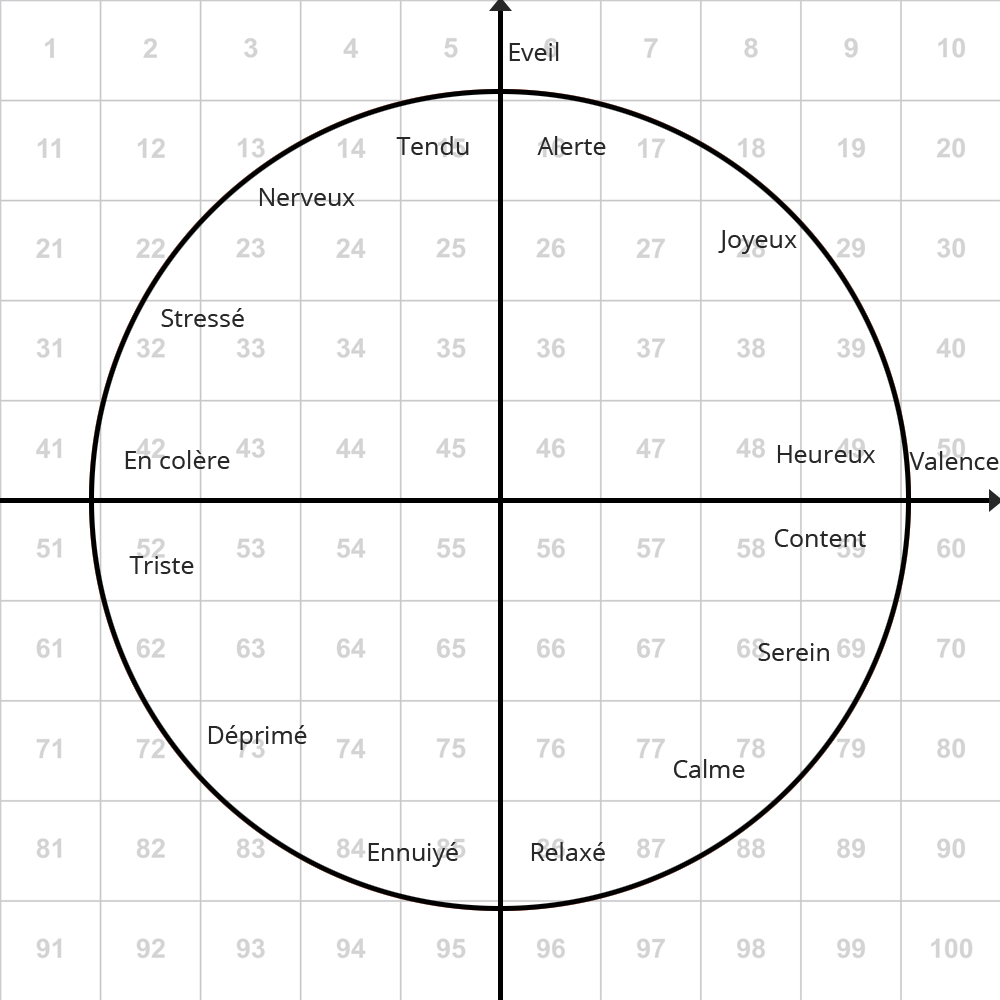
\includegraphics[width=.55\textwidth]{./figure_circumplex_model.png}
    \caption{Grille utilisée pour l'évaluation de l'état émotionnel du participant}
    \label{russel}
\end{figure}

\subsection{Tâche}
La tâche de temps de réaction consistait à cliquer le plus vite possible dès le changement de couleur de l'écran. Dans un premier temps un gros carré noir était affiché avec un petit compteur de trois secondes. A la fin de celui-ci, le carré pouvait passer du noir au rouge dans un intervalle de $ 1 $ à $ 3 $ secondes. Lorsque le participant avait cliqué, un nouvelle essai commencé avec l'affichage du compteur. Le tout était effectué $ 15 $ fois. 

\section{Résultat}
\subsection{Vérification de l'induction émotionnelle}
\begin{figure}[htbp]
    \centering
    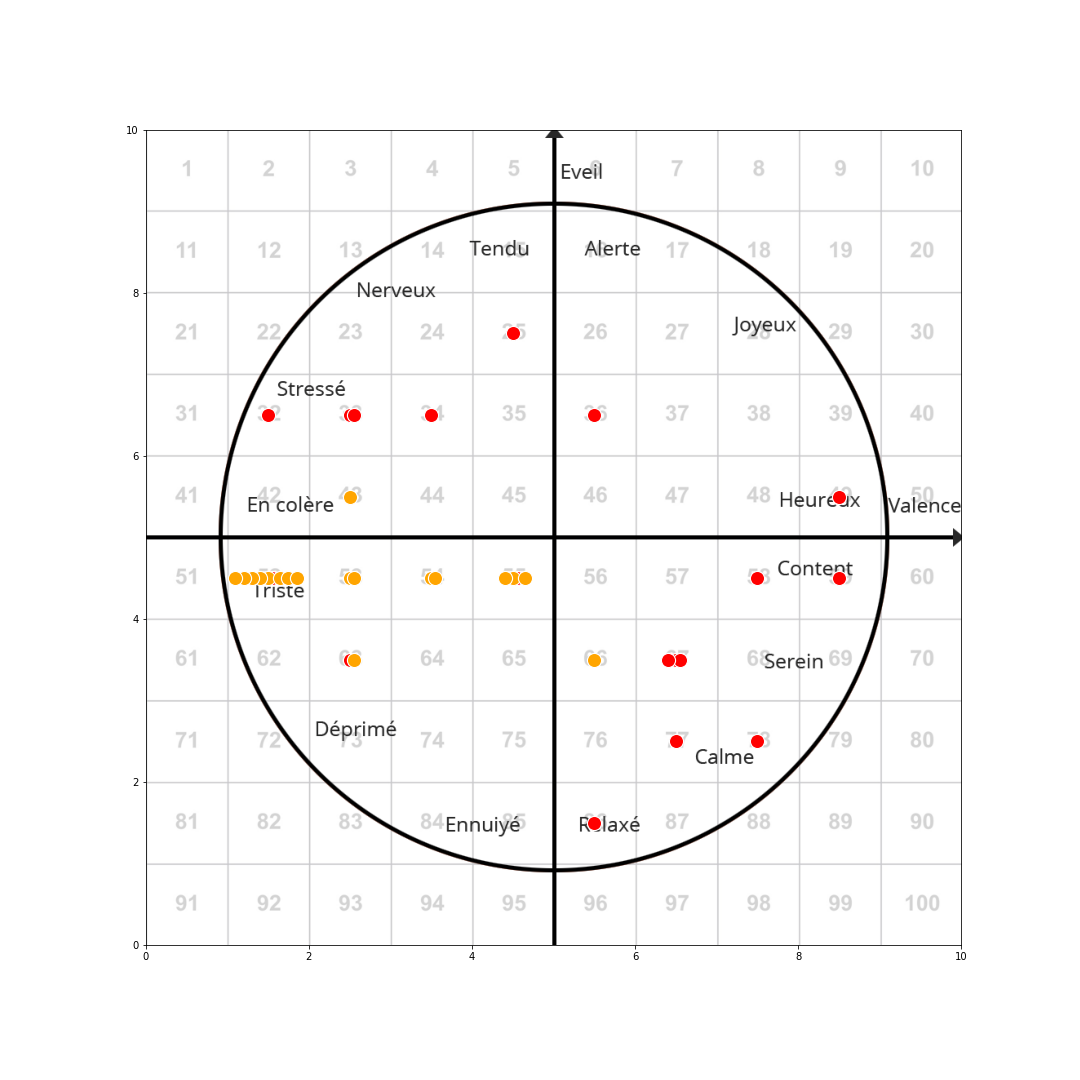
\includegraphics[width=.75\textwidth]{./mood_sad.png}
    \caption{Réponse du groupe "tristesse" au circumplex avant et après l'induction émotionnelle}
    \label{mood_sad}
\end{figure}
La figure \ref{mood_sad} décrit les résultats de l'induction émotionnelle pour le groupe "tristesse". On peut voir une perte de valence notable après le visionnage de la vidéo. De nombreux participants ont coché la case correspondant à la "tristesse" directement.

\begin{figure}[htbp]
    \centering
    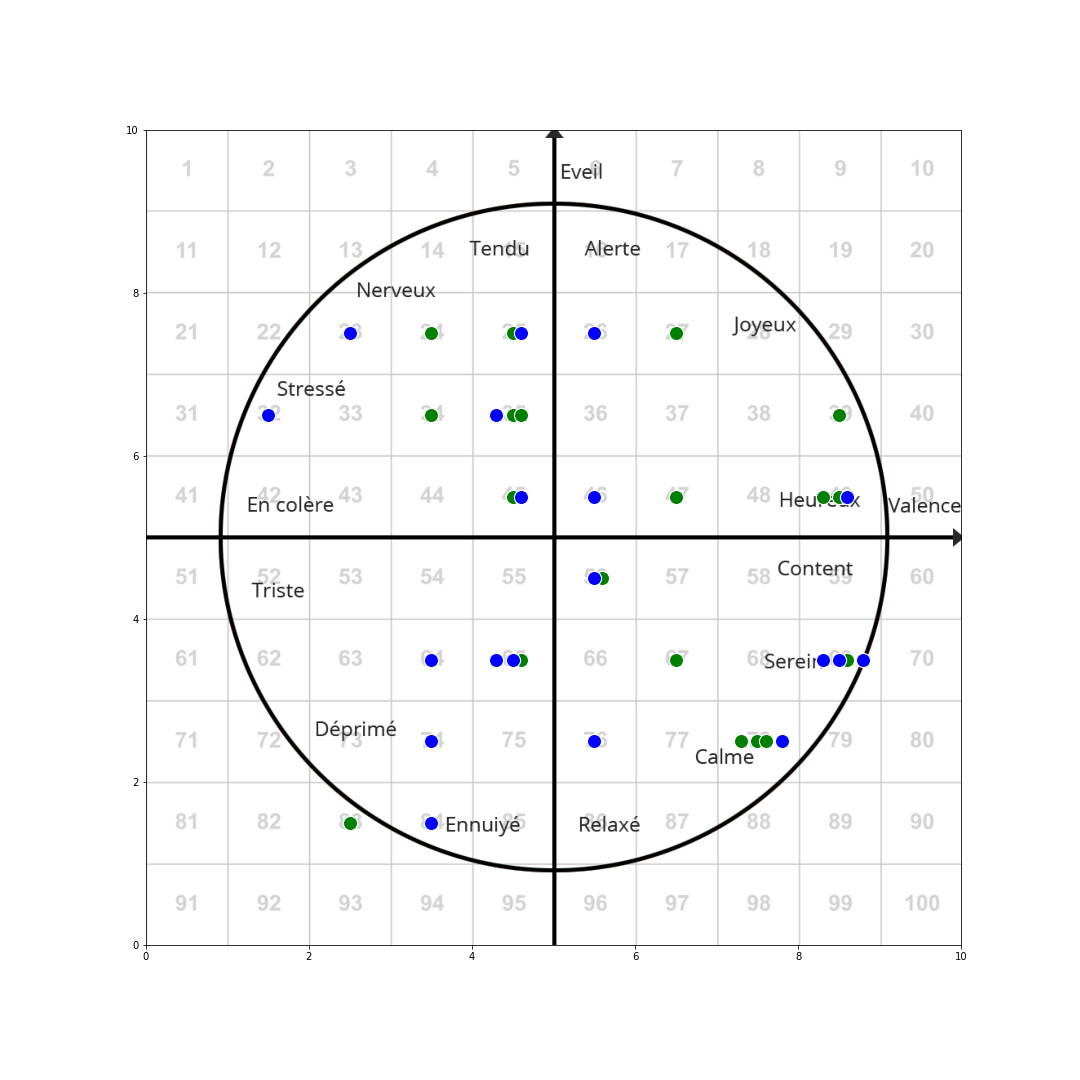
\includegraphics[width=.75\textwidth]{./mood_neutral.png}
    \caption{Réponse du groupe "neutre" au circumplex avant et après l'induction émotionnelle}
    \label{mood_neutral}
\end{figure}
La figure \ref{mood_sad} décrit les résultats de l'induction émotionnelle pour le groupe "neutre". Celle-ci est plus mitigée. En effet, les retours des participants m'ont indiqué que la vidéo était très ennuyeuse créant une baisse de l'éveil chez le ressenti des participants.

\subsection{Effet de l'induction émotionnelle sur le temps de réaction}
\begin{figure}[htbp]
    \centering
    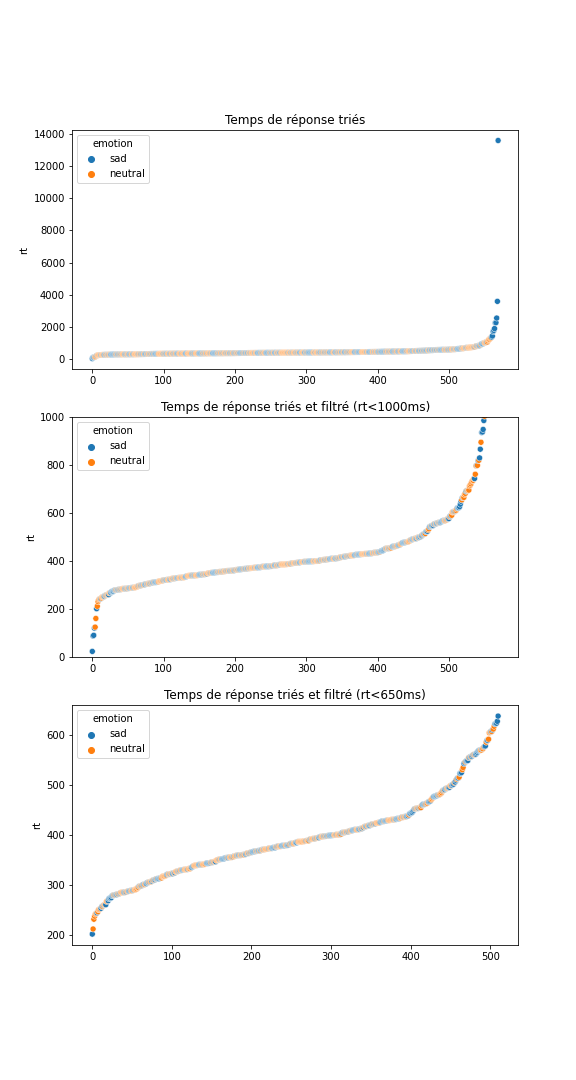
\includegraphics[width=.75\textwidth]{./RT_plot.png}
    \label{RT_plot}
\end{figure}
On peut voir certains temps de réaction aberrant dans la figure \ref{RT_plot}, notamment le 13000ms. Plus globalement, les TRs en dessous de 200ms ne sont pas réalistes (chance par anticipation ou spam click) et ceux au dessus de 650ms peuvent être dû au temps de compréhension de la tache ou à un bug du téléphone.

En prenant la moyenne par participant des TR filtrés, on ne trouve pas de différence significative entre les deux groupes avec un test de Student ($p=0.57$) \\
En revanche, en effectuant le test directement sur la liste des temps de réaction pour les deux groupes, sans faire de moyenne, on obtient cette fois une plus petite p-valeur avec $p=0.064$.

Les visualisations ont été faites sur Python avec la bibliothèque Seaborn et les tests statistiques avec la bibliothèque Scipy.

\section{Conclusion}
Dans cette étude, nous avons pu confirmer la possibilité d'induire une émotion chez le participant par la visualisation d'une vidéo. Mais cette induction émotionnelle reste à quantifier statistiquement.

L'émotion triste induite semble avoir un très faible effet inhibiteur, ici non significatif, sur les temps de réaction. En continuant d'augmenter l'effectif, cela devrait améliorer la significativité. 

La vidéo neutre semble induire un changement dans l'éveil, indiquant qu'elle n'est finalement pas si neutre. C'est un biais qui sera à prendre en compte dans les prochaines études.

Les quelques temps de réaction au dessus de 1000ms peuvent être attribué au côté distanciel de l'expérience. En effet, il n'y a aucune possibilité de vérifier la bonne compréhension de la consigne, les distraction, la vitesse du téléphone. Mais en revanche, cela m'a permis de trouver une quarantaine de participant en quelques jours.


\bibliographystyle{plain} % We choose the "plain" reference style
\bibliography{bib} % Entries are in the refs.bib file
\nocite{*}

\end{document}